Francis Galton wrote in 1907 an article in which he reported an experiment that a crowd of people at an agricultural fair tried to guess the weight of a particular ox. Galton verified that the average of the assumed weights converged to a value very close to the actual weight of the ox and analyzing the distribution of values grounded the Wisdom of the Crowd concept, according to which a heterogeneous crowd large enough tends to provide such a good expert result \cite{GALTON1907}. Additionally, James Surowiecki listed in his book "The Wisdom of the Crowds" \cite{surowiecki2005wisdom} four requirements for a crowd to deliver good results.

\begin{itemize}
\item{\textbf{Diversity:}} each person adds private information or bias.
\item{\textbf{Independence:}} people form their opinions independently.
\item{\textbf{Decentralization:}} people draw on their own knowledge.
\item{\textbf{Aggregation:}} a mechanism exists to turn private judgments into a collective decision.
\end{itemize}

Crowdsourcing platforms are environments suited to this theory, especially because it is possible to reach workers from different parts of the world and contexts with different backgrounds, which favors diversity. A common scenario in these environments involves workers receiving tasks and executing them without interacting with others, which helps create conditions for Independence and Decentralization.

For each task, an appropriate aggregation method should be applied. These methods may involve the convergence of responses, geometric means, contribution merging, as well as other types of processing. In this work, three categories of aggregation methods are also considered: automatic, supervised and manual.


\begin{figure*}[!th]
	\centerline{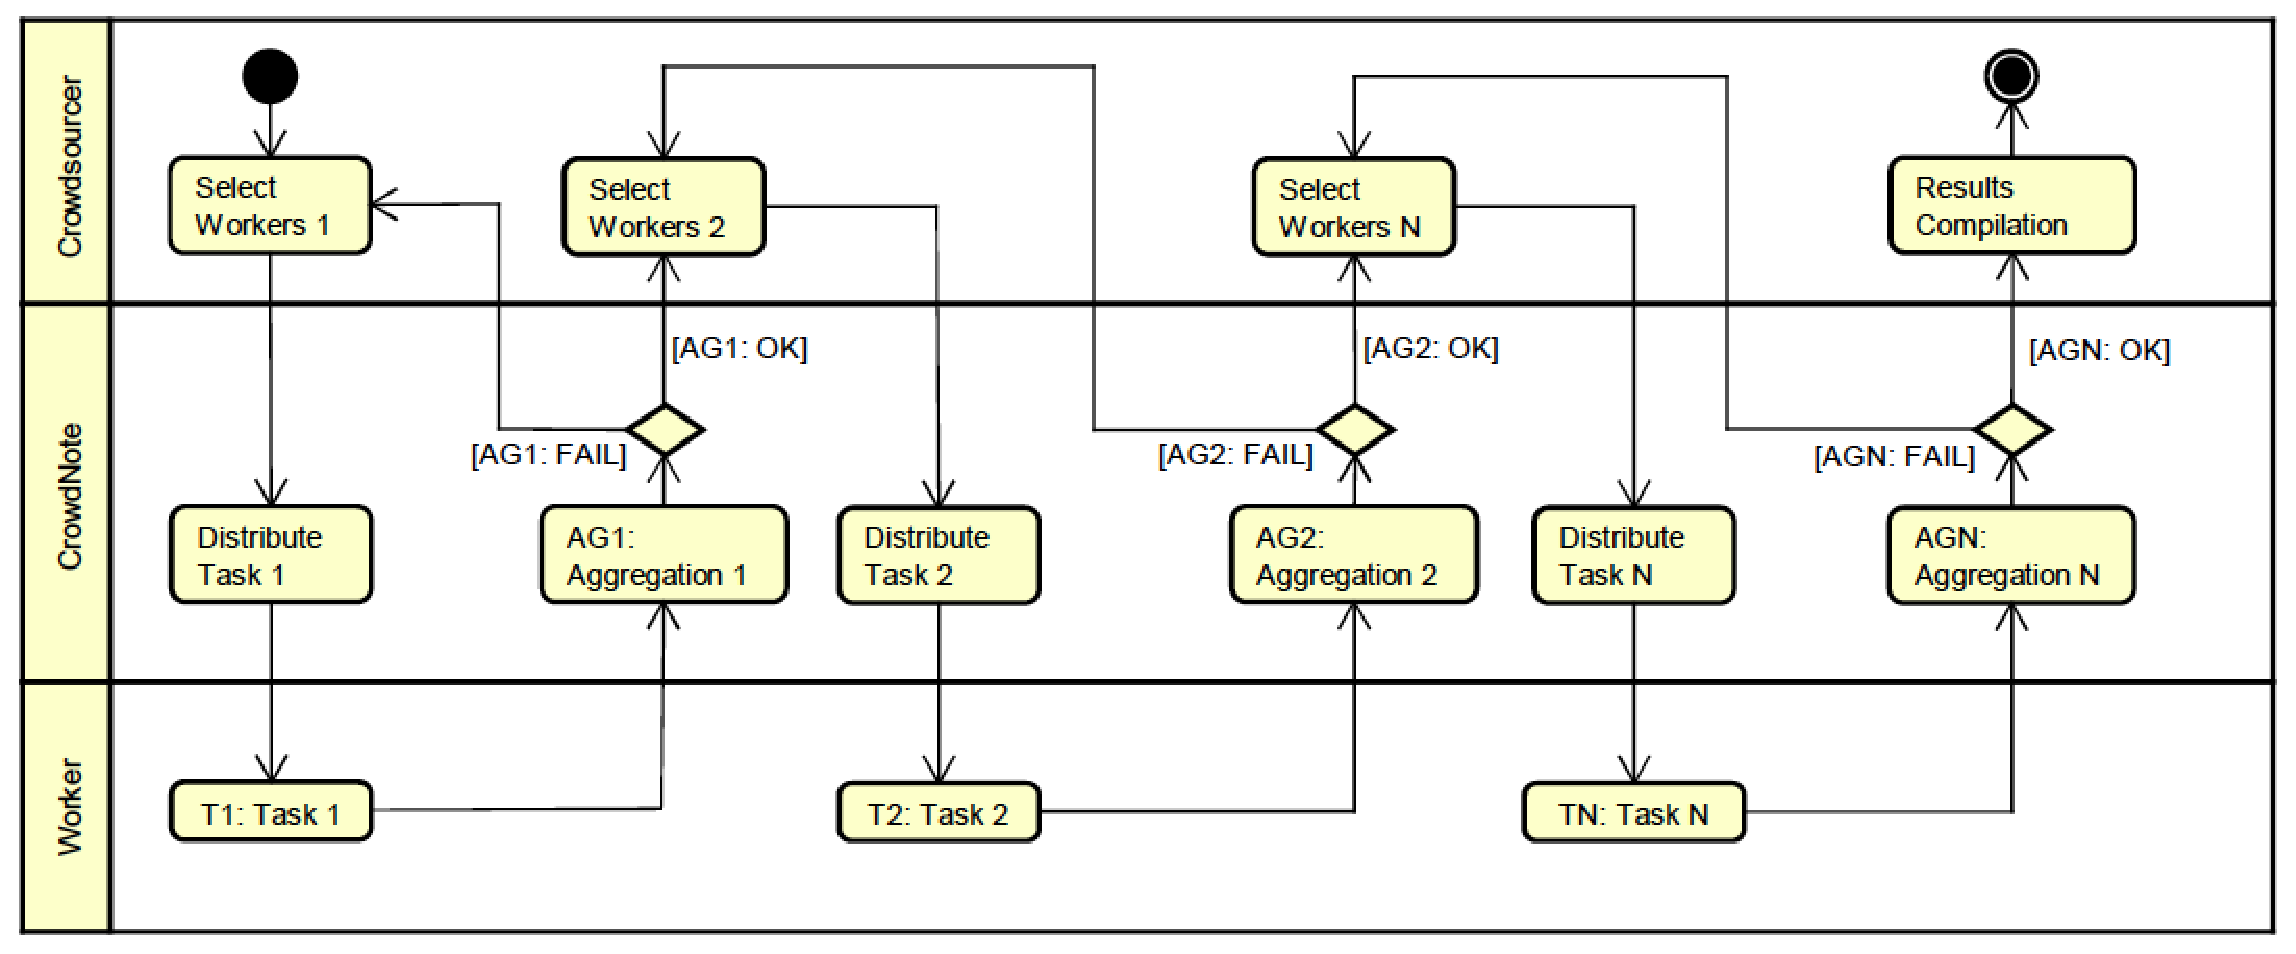
\includegraphics[scale=0.38] {figure/method}}
	\caption{Process workflow. T (Task);  AG (Aggregation).}
	\label{method}
\end{figure*}

\begin{itemize}

\item{\textbf{Automatic:}} an automatic aggregation method employs algorithms to process the contributions in order to generate the desired outcome. This kind of method involves convergence analysis, geometric mean, instance prevalence, and ranking. 

\item{\textbf{Supervised:}} in some cases its possible to apply automatic convergence methods, although it is required additional human verification or some human interaction in the contributions' processing. 

\item{\textbf{Manual:}} manual aggregation is used when it's not possible to define the rules or algorithm that should be followed to generate the outcome. These situations are usually related to subjectivity and emotional aspects that must be analyzed in the contributions to generate the result.

\end{itemize}
